\documentclass[12pt,a4paper]{report}
\usepackage[utf8]{inputenc}
\usepackage[top=1.5cm,bottom=1cm,right=1cm,left=1cm]{geometry}
%\usepackage[margin=1in]{geometry}
\usepackage{amsfonts}
\usepackage{fancybox}
\usepackage{graphicx}
\usepackage{boites}
\usepackage[export]{adjustbox}
\usepackage{float}[H]
\usepackage[french]{babel}
\usepackage{xcolor}
\usepackage{babel}
\usepackage{libertine}
\usepackage{amsmath,amsfonts,amssymb,mathrsfs}
\usepackage{amsthm}
\usepackage{thmtools}
\usepackage{titlesec}
\usepackage{float,lscape}
\usepackage{tikz}
\usepackage[hidelinks]{hyperref}
\hypersetup{
	colorlinks,
	citecolor=black,
	filecolor=black,
	linkcolor= black,
	urlcolor=black}

\renewcommand{\baselinestretch}{1.25}
\usepackage[Bjarne]{fncychap} 

\usepackage{geometry}
\geometry{hmargin=2.5cm,vmargin=2cm}

%-------------------------------------------------------
%%%%%%%%% Mes commandes et environements %%%%%%%%%%%%%%%
%-------------------------------------------------------
\newtheorem {Pro}{Proposition}[section]
\newtheorem{Def}{Définition}[section]
\newtheorem {theo} {Théorème}[section]
\newtheorem {Le} {Lemme}[section]
\newtheorem* {Preuve} {\underline{Preuve}}
\newtheorem {Corollaire} {Corollaire}[section]
\newtheorem* {ex} {\underline{Exemple}}%[section]
\newtheorem* {exc} {\underline{Contre Exemple}}%[section]
\newtheorem* {exs} {\underline{Exemples}}
\newtheorem* {Rq} {Remarque}%[section]
\newtheorem* {Rqs} {Remarques}%[section]
\newtheorem {Prop}{Proposition}[section]
\newtheorem* {Defs}{Définitions}
%\newtheorem{ex}{Exemple}%[section]


\pagestyle{plain}
\usetikzlibrary{backgrounds,shadings,calc}
\colorlet{fff}{white!30!black!40}
\colorlet{ggg}{fff!80!black}
\tikzstyle{a}=[draw=ggg,right color=ggg,left color=ggg!50!black]
\tikzstyle{b}=[draw=ggg,right color=fff,left color=fff!25]
\newdimen\bv
\bv=1.5cm
\def\titlebox#1{%
	\begin{tikzpicture}
		\node[minimum width=0.75\linewidth,align=center,font=\bfseries\huge] (1) {#1};
		\begin{scope}[on background layer]
			\coordinate (a) at($(1.south east)+(-.25\bv,-.25\bv)$);
			\coordinate (b) at($(a)+(.5\bv,0)$);
			\coordinate (e) at($(1.south west)+(.25\bv,.25\bv)$);
			\coordinate (d) at($(1.north west)+(0,.25\bv)$);
			\coordinate (c) at($(d)+(.25\bv,0)$);
			\coordinate (f) at($(d)+(-.25\bv,0)$);
			\path [draw=ggg,right color=fff,left color=fff,middle color=white](f)arc(180:270:.25\bv)--(1.north east)arc(90:0:.25\bv)--(b)arc(0:90:.25\bv)--(1.south west)arc(-90:-180:.25\bv)--cycle;
			\path [a] (d)-|(e)arc(0:-180:.125\bv)--cycle;
			\path [b](c)--(e)arc(0:180:.25\bv)--(f)arc(180:0:.25\bv)--cycle;
			\path [b](a)|-(1.south east)--+(0,-.25\bv)arc(0:180:.125\bv)--cycle;
			\path[a](1.south east)arc(90:-180:.25\bv)arc(180:0:.125\bv)--cycle;
		\end{scope}
	\end{tikzpicture}
}
\def\shape#1{\scalebox{#1}{%
		\begin{tikzpicture}
			\node[circle,fill=cyan!75!fff,inner sep=4mm](5){};
			\foreach \i in {0,1,2}{
				\fill[cyan!75!fff,transform canvas={rotate=-\i*45}](5.east)to[bend left=45]+(3,0)to[bend left=45]cycle;
			}
		\end{tikzpicture}
}}

\def\size{1}


\begin{document}
	\renewcommand{\thepage}{}
	
	\begin{tabular}{ l c r }
		\begin{minipage}{3cm}
			
\includegraphics[width=3cm]{images/ensa}
		\end{minipage}&
		\begin{minipage}{10cm}
			\begin{centering}
				\textbf{Université Sultan Moulay Slimane}\\
				\textbf{ECOLE NATIONALE DES SCIENCES APPLIQUEES}\\
				Département de Mathématiques et Informatique\\
			\end{centering}
		\end{minipage}&
		\begin{minipage}{3cm}
			
\includegraphics[width=2cm]{images/usms}
		\end{minipage}  
	\end{tabular}
	\vglue5mm
	\begin{center}
		
		\vglue3cm\sl
		\underline{\bf\Large PROJET DU DATA MINING}
		\vglue5mm
		\vspace{2cm}
		
		
	\begin{center}
		\begin{tikzpicture}
			\node[align=center,draw,thick,minimum width=\textwidth,inner sep=6mm] (titlebox)%
			{\textsc{\large  CLASSIFICATION METHODES}\\[\baselineskip]\textbf{\huge Support Vector Machines}};
		%	\node[fill=white] (W) at (titlebox.north) {\bfseries \Huge W};
		%	\node (feat) at ([yshift=9mm]titlebox.north) {\textsc{\Large Feature}};
		\end{tikzpicture}
	\end{center}
		
		%\vskip3mm
	%	\titlebox{\huge\bfseries CLASSIFICATION \\METHODES }
%\title{\fbox{Voilà le titre}}
		\large
		
		\vspace*{0.5cm}
		\large
		\begin{flushleft}
			\textit{Réalisé par :\begin{center}
					\Large EL HAMID Youssef\\DRIOUCH Latifa\\DAKIR Ismahane \\
			\end{center}}
		\end{flushleft}  %\\[4mm]
		
		\hspace*{0.5cm} \begin{flushleft}
			\textit{Sous la direction de : \Large Pr. ORDOU Amal}
		\end{flushleft}
		\vspace*{1cm}
		
		
		\vspace{1cm}
		
		
		%\vspace*{3cm}
		
		\begin{flushright}
			{\large Année universitaire : 2022 - 2023}
		\end{flushright}
		
	\end{center}
	
	
	\tableofcontents
	
	%\listoftheorems[ignoreall,show={Pro,definition,theo}]
	\clearpage
	
	\renewcommand{\thepage}{\arabic{page}}
	\setcounter{page}{1}
	
	\chapter*{INTRODUCTION    }
	\addcontentsline{toc}{chapter}{INTRODUCTION}
	\large
	L'apprentissage automatique est un domaine de l'informatique qui a connu une croissance rapide ces dernières années, offrant des techniques permettant aux machines d'apprendre à partir de données et d'effectuer des tâches complexes sans être explicitement programmées. Les algorithmes d'apprentissage supervisé, en particulier la classification, sont largement utilisés dans divers domaines tels que la reconnaissance d'images, la biologie, la finance et bien d'autres encore. Les SVM (Support Vector Machines) sont l'un des algorithmes de classification les plus populaires utilisés dans l'apprentissage automatique en raison de leur capacité à gérer les problèmes de classification linéaire et non linéaire. Les SVM sont particulièrement utiles dans les situations où les données d'entraînement sont complexes et le bruit est important. Dans ce rapport, nous présentons une étude sur l'utilisation de SVM pour la classification de données de spam et de non-spam. Nous discuterons des principes de base de SVM, de leur fonctionnement, de leur entraînement, de leur validation et de leur application pour la classification de données de spam et de non-spam. Nous montrerons comment les SVM peuvent être utilisés pour améliorer la précision de la classification, tout en minimisant les faux positifs et les faux négatifs.
	
	\newpage
	
	
	\chapter{Principe  et cas d'utilisation}
	Le principe des SVM consiste à ramener un problème de classification ou de discrimination à un hyperplan (feature space) dans lequel les données sont séparées en plusieurs classes dont la frontière est la plus éloignée possible des points de données (ou "marge maximale"). D'où l'autre nom attribué aux SVM : les séparateurs à vaste marge. Le concept de frontière implique que les données soient linéairement séparables. Pour y parvenir, les support vector machines font appel à des noyaux, c'est-à-dire des fonctions mathématiques permettant de projeter et séparer les données dans l'espace vectoriel, les "vecteurs de support" étant les données les plus proches de la frontière. C'est la frontière la plus éloignée de tous les points d'entraînement qui est optimale, et qui présente donc la meilleure capacité de généralisation. \\
	
	
	Les cas d'utilisation de la méthode SVM sont très variés et couvrent de nombreux domaines, tels que la reconnaissance de caractères manuscrits, la détection de fraude bancaire, la prédiction de la qualité de l'air, la détection de cancer et bien d'autres encore.
	
	En reconnaissance de caractères manuscrits, la méthode SVM est utilisée pour identifier les caractères dans une image numérique en se basant sur un ensemble d'exemples d'images pré-classifiées. Dans le domaine de la détection de fraude bancaire, la méthode SVM est utilisée pour identifier les transactions suspectes et les activités frauduleuses en se basant sur des schémas d'activités frauduleuses connus.
	
	Dans le domaine de la prédiction de la qualité de l'air, la méthode SVM est utilisée pour prédire les niveaux de pollution de l'air en se basant sur des données historiques de qualité de l'air et des données météorologiques. Dans le domaine de la détection de cancer, la méthode SVM est utilisée pour identifier les tumeurs cancéreuses dans des images radiographiques en se basant sur un ensemble d'exemples pré-classifiés.
	
	En somme, la méthode SVM est utilisée dans de nombreux domaines pour résoudre des problèmes de classification et de régression. Son utilisation est très répandue dans les domaines de la reconnaissance de formes, de la vision par ordinateur et de la bioinformatique, mais elle trouve également des applications dans des domaines tels que la finance, l'environnement et la médecine.
	
	
	
	\newpage
	
	\chapter{SVMs binaires }
	\section{Cas linéairement séparable}
	Le cas le plus simple est celui où les données d’entrainement viennent uniquement de
	deux classes différentes (+1 ou -1), on parle alors de classification binaire. L’idée des SVMs
	est de rechercher un hyperplan (droite dans le cas de deux dimensions) qui sépare le mieux
	ces deux classes. Si un tel hyperplan existe, c’est-à-dire si les données sont linéairement
	séparables, on parle d’une machine à vecteur support à marge dure (Hard margin).
	L’hyperplan séparateur est représenté par l’équation suivante :\begin{center}
	$ 	H(x) = w^{T} x + b $
	\end{center}
	Où w est un vecteur de m dimensions et b est un terme. La fonction de décision, pour un
	exemple x, peut être exprimée comme suit :
	\begin{center}
		$ Classe = 1 \quad Si\; H(x) > 0 $\\
		$ Classe = -1 \quad Si\; H(x) < 0 $
	\end{center}
Puisque les deux classes sont linéairement séparables, il n’existe aucun exemple qui se
situe sur l’hyperplan, c-à-d qui satisfait $ H(x) = 0 $. Il convient alors d’utiliser la fonction
de décisions suivante :
\begin{center}
	$ Classe = 1 \quad Si\; H(x) > 1 $\\
$ 	Classe = -1 \quad Si\; H(x) < -1 $
\end{center}
Les valeurs +1 et -1 à droite des inégalités peuvent être des constantes quelconques +a et
-a, mais en divisant les deux parties des inégalités par a, on trouve les inégalités précédentes
qui sont équivalentes à l’équation suivante :\begin{center}
	$ y_{i}(w^{T} x_{i} + b) \geq 1; i = 1::n $
\end{center}
L’hyperplan $ w^{T} x+b = 0 $ représente un hyperplan séparateur des deux classes, et la distance
entre cet hyperplan et l’exemple le plus proche s’appelle la marge. La région qui se trouve entre les deux hyperplans $ w^{T} x + b = -1 $ et $ w^{T} x + b = +1 $ est appelée la région de
généralisation de la machine d’apprentissage. Plus cette région est importante, plus est la
capacité de généralisation de la machine. La maximisation de cette région est l’objectif de
la phase d’entrainement qui consiste, pour la méthode SVM, à rechercher l’hyperplan qui
maximise la région de généralisation c-à-d la marge. Un tel hyperplan est appelé "hyperplan
de séparation optimale". En supposant que les données d’apprentissage ne contiennent pas
des données bruitées (mal-étiquetées) et que les données de test suivent la même probabilité
que celle des données d’entraînement, l’hyperplan de marge maximale va certainement
maximiser la capacité de généralisation de la machine d’apprentissage.\\
La détermination de l’hyperplan optimal passe par la détermination de la distance
euclidienne minimale entre l’hyperplan et l’exemple le plus proche des deux classes. Puisque
le vecteur w est orthogonal sur l’hyperplan séparateur, la droite parallèle à w et reliant un
exemple x à l’hyperplan est donnée par la formule :\begin{center}
	$ \dfrac{aw}{\Arrowvert w \Arrowvert}	+ x = 0 $
\end{center}
Où a représente la distance entre x et l’hyperplan. La résolution de cette équation, donne :\begin{center}
	$ a = -\dfrac{w^{T} x + b}{\Arrowvert w \Arrowvert} $

\end{center}
La distance de tout exemple de l’hyperplan doit être supérieure ou égale à la marge $ \delta  $:
\begin{center}
	$ \dfrac{y_{i}(w^{T} x_{i} + b)}{\Arrowvert w \Arrowvert}\geq\delta $
\end{center}
Si une paire $ (w; b) $ est une solution alors $ (aw; ab) $ est une solution aussi où a est un scalaire.
On impose alors la contrainte suivante :\begin{center}
	$ \Arrowvert w \Arrowvert \delta \geq 1 $
\end{center}
Pour trouver l’hyperplan séparateur qui maximise la marge, on doit déterminer, à partir
des deux dernières inégalités, le vecteur w qui possède la norme euclidienne minimale et
qui vérifie la contrainte de l’équation, de bonne classification des exemples d’entrainement.
L’hyperplan séparateur optimal peut être obtenu en résolvant le problème de l’équation :\begin{center}
	$$
	\left\{\begin{array}{l}
		 Minimiser\; \frac{1}{2} \;\Arrowvert w \Arrowvert^{2} \\
		 sous\; contraintes\\
		 y_{i}(w^{T} x_{i} + b) \geq 1 \forall i = 1..n
	\end{array}\right.
	$$
\end{center}
Remarquons que nous pouvons obtenir le même hyperplan même en supprimant toutes les
données qui vérifient l’inégalité de la contrainte. Les données qui vérifient l’égalité de la contrainte s’appellent les vecteurs supports, et ce sont ces données seules qui contribuent
à la détermination de l’hyperplan. Dans la figure, les données qui se trouvent sur les deux
droites +1 et -1 représentent les vecteurs supports.\\
Le problème de l’équation est un problème de programmation quadratique avec contraintes
linéaires. Dans ce problème, les variables sont w et b, c-à-d que le nombre de variables est
égal à m + 1. Généralement, le nombre de variables est important ce qui ne permet pas
d’utiliser les techniques classiques de programmation quadratique. Dans ce cas le problème
est convertit en un problème dual équivalent sans contraintes de l’équation suivante qui
introduit les multiplicateurs de Lagrange :\begin{center}
	$ Q(w; b;\alpha ) =\frac{1}{2}w^{T}w - \sum_{i=1}^{n}\alpha_{i}(y_{i}(w^{T} x_{i} + b) - 1) $
\end{center}
O$\grave{u}$ les $\alpha_{i}$ sont les multiplicateurs non négatifs de Lagrange. L’optimum de la fonction
objective Q peut être obtenu en la minimisant par rapport à w et b et en la maximisant
par rapport aux $\alpha_{i}$. A l’optimum de la fonction objective, ses dérivées par rapports aux
variables w et b s'annulent ainsi que le produit des $\alpha_{i}$ aux contraintes :
$$
\begin{cases}\frac{\partial Q(w, b, \alpha)}{\partial w}=0 & (a) \\ \frac{\partial Q(w, b, \alpha)}{\partial b}=0 & (b) \\ \alpha_{i}\left\{y_{i}\left(w^{T} x_{i}+b\right)-1\right\}=0 & (c) \\ \alpha_{i} \geq 0 & (d)\end{cases}
$$

De (a) on déduit :

$$
\left\{\begin{array}{l}
	w=\sum_{i=1}^{n} \alpha_{i} y_{i} x_{i} \\
	\sum_{i=1}^{n} \alpha_{i} y_{i}=0
\end{array}\right.
$$

En remplaçant dans la fonction objective, on obtient le problème dual à maximiser suivant :

$$
\begin{cases}\text { Maximiser } & Q(\alpha)=\sum_{i=1}^{n} \alpha_{i}-\sum_{i=1}^{n} \sum_{j=1}^{n} \alpha_{i} \alpha_{j} y_{i} y_{j} x_{i}^{T} x_{j} \\ \text { Sous contraintes } & \\ & \sum_{i=1}^{n} \alpha_{i} y_{i}=0 \\ & \alpha_{i} \geq 0\end{cases}
$$

Si le problème de classification est linéairement séparable, une solution optimale pour les $\alpha_{i}$ existe. Les exemples ayant des $\alpha_{i} \neq 0$ représentent les vecteurs supports appartenant aux deux classes. La fonction de décision est donnée par :

$$
H(x)=\sum_{S} \alpha_{i} y_{i} x^{T} x_{i}+b
$$

Où $S$ représente l'ensemble des vecteurs supports. $b$ peut être calculé à partir de n'importe quel vecteur support par l'équation :

$$
b=y_{i}-w^{T} x_{i}
$$

D'un point de vue précision, on prend la moyenne de $b$ pour tous les vecteurs supports :

$$
b=\frac{1}{|S|} \sum_{i \in S} y_{i}-w^{T} x_{i}
$$

La fonction de décision $\mathrm{H}$ peut être calculée, donc, pour chaque nouvel exemple $x$ par la fonction $H(x)$ et la décision peut être prise comme suit :
\begin{center}
$$
\begin{cases}x\in classe + 1\; si \;H(x)>0 \\ x\in classe - 1\; si \;H(x)<0 \\  x\;inclassifiable\; si \;H(x)=0\end{cases}
$$
\end{center}

La zone $-1<H(x)<1$ est appelée la zone de généralisation.
Si on prend un exemple $x_{k}$ de l'ensemble d'entrainement appartenant à la classe $y_{k}$ et on calcule sa fonction de décision $H\left(x_{k}\right)$, on peut se trouver dans l'un des cas suivants :

\begin{enumerate}
	\item $y_{k} * H\left(x_{k}\right)>1$ : dans ce cas l'exemple est bien classé et ne se situe pas dans la zone de la marge. Il ne représente pas un vecteur support.
	
	\item $y_{k} * H\left(x_{k}\right)=1$ : dans ce cas l'exemple est bien classé et se situe aux frontières de la zone de la marge. Il représente un vecteur support.
	
	\item $0<y_{k} * H\left(x_{k}\right)<1$ : dans ce cas l'exemple est bien classé et se situe dans de la zone de la marge. Il ne représente pas un vecteur support.
	
	\item $y_{k} * H\left(x_{k}\right)<0$ : dans ce cas l'exemple se situe dans le mauvais coté, il est mal classé et ne représente pas un vecteur support.
	
\end{enumerate}

\section{Cas non linéairement séparable}
En réalité, un hyperplan séparateur n'existe pas toujours, et même s'il existe, il ne représente pas généralement la meilleure solution pour la classification. En plus une erreur d'étiquetage dans les données d'entrainement (un exemple étiqueté +1 au lieu de -1 par exemple) affectera crucialement l'hyperplan.

Dans le cas où les données ne sont pas linéairement séparables, ou contiennent du bruit (outliers : données mal étiquetées) les contraintes ne peuvent être vérifiées, et il y a nécessité de les relaxer un peu. Ceci peut être fait en admettant une certaine erreur de classification des données ce qui est appelé "SVM à marge souple (Soft Margin)".

\begin{figure}[!ht]
	\centering
	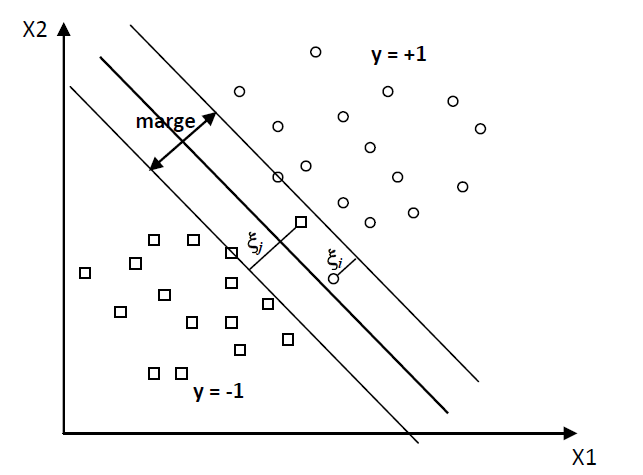
\includegraphics[width=10cm]{images/capt1}
	\caption{SVM binaire à marge souple.}
\end{figure}

On introduit alors sur les contraintes des variables $\xi_{i}$ dites de relaxation pour obtenir la contrainte de l'équation :
$$
y_{i}\left(w^{T} x_{i}+b\right) \geq 1-\xi_{i}, i=1 . . n
$$
Grâce aux variables de relaxation non négatives $\xi_{i}$, un hyperplan séparateur existera toujours.

Si $\xi_{i}<1, x_{i}$ ne respecte pas la marge mais reste bien classé, sinon $x_{i}$ est mal classé par l'hyperplan. Dans ce cas, au lieu de rechercher uniquement un hyperplan séparateur qui maximise la marge, on recherche un hyperplan qui minimise aussi la somme des erreurs permises c-à-d minimiser $Q(w)=\sum_{i=1}^{n} \xi_{i}$.
Le problème dual devient donc :
$$
\begin{cases}\text { Minimiser } & \frac{1}{2}\|w\|^{2}+C \sum_{i=1}^{n} \xi_{i} \\ \text { sous contraintes } \\ y_{i}\left(w^{T} x_{i}+b\right) \geq 1-\xi_{i} & i=1 . . n \\ \xi_{i} \geq 0 & \end{cases}
$$

Où $\mathrm{C}$ est un paramètre positif libre (mais fixe) qui représente une balance entre les deux termes de la fonction objective (la marge et les erreurs permises) c-à-d entre la maximisation de la marge et la minimisation de l'erreur de classification. On obtient le problème dual de l'équation suivante où on introduit les multiplicateurs de Lagrange $\alpha_{i}$ et $\beta_{i}$ :
$$
Q(w, b, \alpha, \xi, \beta)=\frac{1}{2} w^{T} w+C \sum_{i=1}^{n} \xi_{i}-\sum_{i=1}^{n} \alpha_{i} y_{i}\left(w^{T} x_{i}+b\right)-1+\xi_{i}-\sum_{i=1}^{n} \beta_{i} \xi_{i}
$$

À la solution optimale, les dérivées par rapport aux variables $w, b, \alpha, \beta$ s'annulent ainsi que le produit des contraintes aux multiplicateurs. Les conditions suivantes sont alors vérifiées :

$$
\begin{cases}\frac{\partial Q(w, b, \xi, \alpha, \beta)}{\partial w}=0 & (a) \\ \frac{\partial Q(w, b, \xi, \alpha, \beta)}{\partial b}=0 & (b) \\ \alpha_{i}\left\{y_{i}\left(w^{T} x_{i}+b\right)-1+\xi_{i}\right\}=0 & (c) \\ \beta_{i} \xi_{i}=0 & (d) \\ \alpha_{i} \geq 0 ; \beta_{i} \geq 0 ; \xi_{i} \geq 0 & (e)\end{cases}
$$
On déduit :
$$
\left\{\begin{array}{l}
	w=\sum_{i=1}^{n} \alpha_{i} y_{i} x_{i} \\
	\sum_{i=1}^{n} \alpha_{i} y_{i}=0 \\
	\alpha_{i}+\beta_{i}=0
\end{array}\right.
$$
En remplaçant cette équation dans la fonction objective, on obtient le problème dual suivant :
$$
\begin{cases}\text { Maximiser } & Q(\alpha)=\sum_{i=1}^{n} \alpha_{i}-\frac{1}{2} \sum_{i=1}^{n} \sum_{j=1}^{n} \alpha_{i} \alpha_{j} y_{i} y_{j} x_{i}^{T} x_{j} \\ \text { sous contraintes } & \\ & \sum_{i=1}^{n} \alpha_{i} y_{i}=0 \\ & 0 \leq \alpha_{i} \leq C\end{cases}
$$
La seule différence avec la SVM à marge dure est que les $\alpha_{i}$ ne peuvent pas dépasser C, ils peuvent être dans l'un des trois cas suivants :
\begin{enumerate}
	\item $\alpha_{i}=0 \Rightarrow \beta_{i}=C \Rightarrow \xi_{i}=0: x_{i}$ est bien classé,
	
	\item $0<\alpha_{i}<C \Rightarrow \beta_{i}>0 \Rightarrow \xi_{i}=0 \Rightarrow y_{i}\left(w^{T} x_{i}+b\right)=1: x_{i}$ est un vecteur support et est appelé dans ce cas vecteur support non borné (unbounded),
	
	\item $\alpha_{i}=C \Rightarrow \beta_{i}=0 \Rightarrow \xi_{i} \geq 0 \Rightarrow y_{i}\left(w^{T} x_{i}+b\right)=1-\xi_{i}: x_{i}$ est un vecteur support appelé dans ce cas vecteur support borné (bounded). Si $0 \leq \xi_{i}<1, x_{i}$ est bien classé, sinon $x_{i}$ est mal classé.
	
\end{enumerate}
Ces conditions sur les $\alpha_{i}$ sont appelées les conditions de Karush-Kuhn-Tucker (KKT), elles sont très utilisées par les algorithmes d'optimisation pour rechercher les $\alpha_{i}$ optimums et par conséquent l'hyperplan optimal. La fonction de décision est alors calculée de la même manière que dans le cas des SVMs à marge dure mais uniquement à base des vecteurs supports non bornés par :
$$
H(x)=\sum_{i \in U} \alpha_{i} y_{i} x_{i}^{T} x+b
$$
Pour les vecteurs supports non bornés, nous avons :
$$
b=y_{i}-w^{T} x_{i}
$$
Pour garantir une bonne précision, on prend la moyenne de $b$ pour tous les vecteurs supports non bornés :
$$
b=\frac{1}{|U|} \sum_{i \in U} y_{i}-w^{T} x_{i}
$$
\subsection{Utilisation des noyaux}
Le fait d'admettre la mal-classification de certains exemples, ne peut pas toujours donner une bonne généralisation pour un hyperplan même si ce dernier est optimisé.

\begin{figure}[!ht]
	\centering
	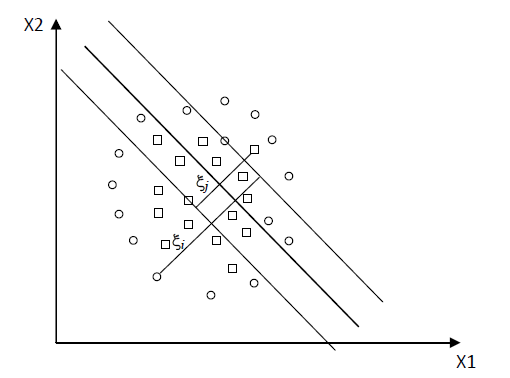
\includegraphics[width=9.5cm]{images/capt2}
	%\caption{SVM binaire à marge souple.}
\end{figure}
Plutôt qu’une droite, la représentation idéale de la fonction de décision serait une
représentation qui colle le mieux aux données d’entrainement.
\begin{figure}[!ht]
	\centering
	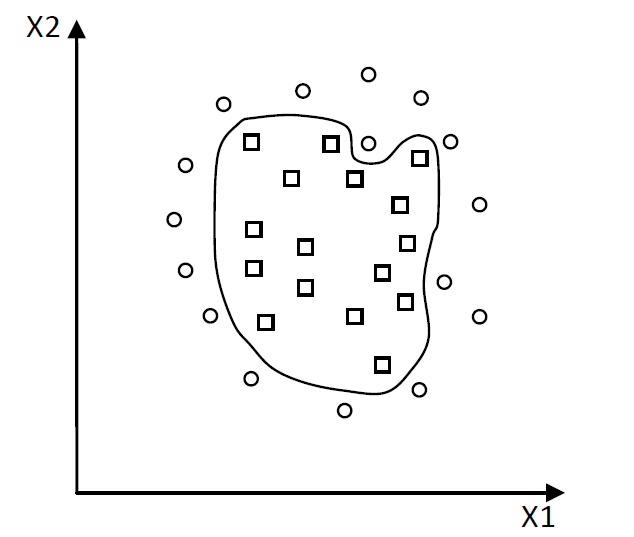
\includegraphics[width=8.5cm]{images/capt3}
	\caption{Représentation idéale de la fonction de décision}
\end{figure}



La détermination d'une telle fonction non linéaire est très difficile voire impossible. Pour cela les données sont amenées dans un espace où cette fonction devient linéaire, cette astuce permet de garder les mêmes modèles de problèmes d'optimisation vus dans les sections précédentes, utilisant les SVMs basées essentiellement sur le principe de séparation linéaire. Cette transformation d'espace est réalisée souvent à l'aide d'une fonction $F=\{\phi(x) \mid x \in X\}$ appelé "Mapping function" et le nouvel espace est appelé espace de caractéristiques "Features space".

Dans ce nouvel espace de caractéristiques, la fonction objective à optimiser devient :

$$
Q(\alpha)=\sum_{i=1}^{n} \alpha_{i}-\frac{1}{2} \sum_{i=1}^{n} \sum_{j=1}^{n} \alpha_{i} \alpha_{j} y_{i} y_{j}\left\langle\phi\left(x_{i}\right), \phi\left(x_{j}\right)\right\rangle
$$

Où $\left\langle\phi\left(x_{i}\right), \phi\left(x_{j}\right)\right\rangle$ est le produit scalaire des deux images des vecteurs $x_{i}$ et $x_{j}$ dans le nouvel espace et dont le résultat est un scalaire.
Dans le calcul de l'optimum de la fonction, on utilise une astuce appelée "Noyau" ("Ker$\left.n e l^{\prime \prime}\right)$, au lieu de calculer $\phi\left(x_{i}\right), \phi\left(x_{j}\right)$ et leur produit scalaire, on calcule plutôt une fonction $K\left(x_{i}, x_{j}\right)$ qui représente à la fois les deux transformations (qui peuvent être inconnues) et leur produit scalaire. Cette fonction permet de surmonter le problème de détermination de la transformation $\phi$ et permet d'apprendre des relations non linéaires par des machines linéaires. En pratique, il existe certains noyaux qui sont très utilisés et qui sont considérés comme standards. Une fois le noyau choisi, la fonction objective peut être calculée comme suit :
$$
Q(\alpha)=\sum_{i=1}^{n} \alpha_{i}-\frac{1}{2} \sum_{i=1}^{n} \sum_{j=1}^{n} \alpha_{i} \alpha_{j} y_{i} y_{j} K\left(x_{i}, x_{j}\right)
$$
Et la fonction de décision devient :
$$
H(x)=\sum_{i \in S} \alpha_{i} y_{i} K\left(x_{i}, x\right)+b
$$
Où $S$ représente l'ensemble des vecteurs supports.

\subsection{Exemples de noyaux}
\begin{itemize}
	\item Noyau linéaire: Si les données sont linéairement séparables, on n'a pas besoin de changer d'espace, et le produit scalaire suffit pour définir la fonction de décision :
\end{itemize}
$$
K\left(x_{i}, x_{j}\right)=x_{i}^{T} x_{j}
$$
\begin{itemize}
	\item Noyau polynomial : Le noyau polynomial élève le produit scalaire à une puissance naturelle $d$ :
\end{itemize}
$$
K\left(x_{i}, x_{j}\right)=\left(x_{i}^{T} x_{j}\right)^{d}
$$
Si $d=1$ le noyau devient linéaire. Le noyau polynomial dit non homogène $K\left(x_{i}, x_{j}\right)=$ $\left(x_{i}^{T} x_{j}+C\right)^{d}$ est aussi utilisé.

\begin{itemize}
	\item Noyau RBF : Les noyaux RBF (Radial Basis functions) sont des noyaux qui peuvent être écrits sous la forme : $K\left(x_{i}, x_{j}\right)=f\left(d\left(x_{i}, x_{j}\right)\right)$ où $d$ est une métrique sur $X$ et $f$ est une fonction dans $\Re$. Un exemple des noyaux RBF est le noyau Gaussien :
\end{itemize}
$$
K\left(x_{i}, x_{j}\right)=e^{\left(-\frac{\left\|x_{i}-x_{j}\right\|^{2}}{2 \sigma^{2}}\right)}
$$
Où $\sigma$ est un réel positif qui représente la largeur de bande du noyau.

	\chapter{SVMs multiclasse }
Les machines à vecteur support sont dans leur origine binaires. Cependant, les problèmes
du monde réel sont dans la plupart des cas multiclasse, l’exemple le plus simple en
est la reconnaissance des caractères optiques (OCR). Dans de tels cas, on ne cherche pas à
affecter un nouvel exemple à l’une de deux classes mais à l’une parmi plusieurs, c-à-d que
la décision n’est plus binaire et un seul hyperplan ne suffit plus.
Les méthodes des machines à vecteur support multiclasse, réduisent le problème multiclasse à une composition de plusieurs hyperplans biclasses permettant de tracer les
frontières de décision entre les différentes classes. Ces méthodes décomposent l’ensemble
d’exemples en plusieurs sous ensembles représentant chacun un problème de classification
binaire. Pour chaque problème un hyperplan de séparation est déterminé par la méthode
SVM binaire. On construit lors de la classification une hiérarchie des hyperplans binaires
qui est parcourue de la racine jusqu’à une feuille pour décider de la classe d’un nouvel
exemple. On trouve dans la littérature plusieurs méthodes de décomposition :
\section{Une-contre-reste}
C’est la méthode la plus simple et la plus ancienne. Selon la formulation de Vapnik,
elle consiste à déterminer pour chaque classe k un hyperplan Hk(wk; bk) la séparant de
toutes les autres classes. Cette classe k est considérée comme étant la classe positive (+1)
et les autres classes comme étant la classe négative (-1), ce qui résulte, pour un problème
à K classes, en K SVM binaires. Un hyperplan Hk est défini pour chaque classe k par la
fonction de décision suivante :
\begin{center}
	$\begin{aligned} H_k(x) & =\operatorname{signe}\left(\left\langle w_k, x\right\rangle+b_k\right) \\ & =\left\{\begin{array}{lll}+1 & \text { si } & f_k(x)>0 \\ 0 & \text { sinon }\end{array}\right.\end{aligned}$
\end{center}
La valeur retournée de l’hyperplan permet de savoir si x appartient à la classe k ou non.
Dans le cas où il n’appartient pas à $ k (H_{k}(x) = 0) $, nous n’avons aucune information sur
l’appartenance de x aux autres classes. Pour le savoir, on présente x à tous les hyperplans,
ce qui donne la fonction de décision de l’équation suivante :
\begin{center}
	$k^*=\underbrace{\operatorname{Arg}}_{(1 \leq k \leq K)} \operatorname{Max}\left(H_k(x)\right)$
\end{center}
Si une seule valeur $ H_{k}(x) $ est égale à 1 et toutes les autres sont égales à 0, on conclut que x
appartient à la classe k. Le problème est que l’équation peut être vérifiée pour plus d’une classe, ce qui produit des régions d’ambiguïté, et l’exemple x est dit non classifiable. La figure suivante représente un cas de séparation de 3 classes.
\begin{figure}[!ht]
	\centering
	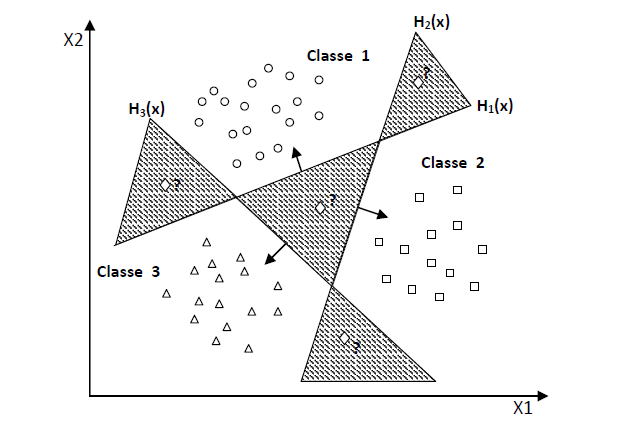
\includegraphics[width=10cm]{images/capt4}
	\caption{Approche une-contre-reste avec des zones d’indécision}
\end{figure}
Pour surmonter cette situation, la méthode 1vsR utilise le principe de "le gagnant prend
tout" ("winner-takes-all") : la classe k retenue est celle qui maximise $ f_{k}(x) = \langle w_{k}; x_{i}\rangle + b_{k} $
de l’équation :
\begin{center}
	$k^*=\underbrace{\operatorname{Arg}}_{(1 \leq k \leq K)} \operatorname{Max}\left(\langle w_{k}; x_{i}\rangle + b_{k}\right)$
\end{center}
Géométriquement interprétée, tout nouvel exemple x est affecté à la classe dont l’hyperplan
est le plus loin de x, parmi les classes ayant H(x) = 1.
\newpage
\begin{figure}[!ht]
	\centering
	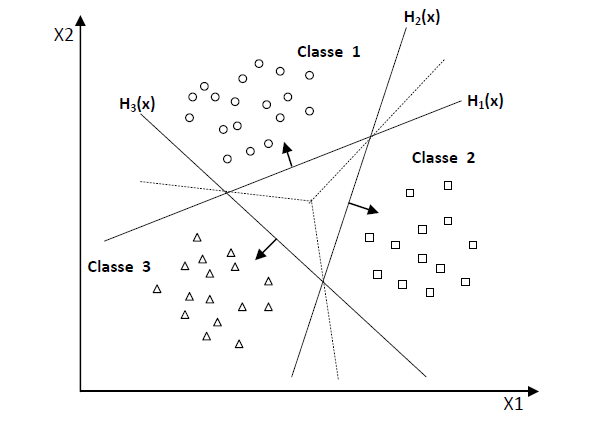
\includegraphics[width=10cm]{images/capt5}
	\caption{Résolution des cas d’indécision dans la méthode 1vsR}
\end{figure}
La méthode 1vsR peut être utilisée pour découvrir même les cas de rejet où un exemple n’appartient à aucune des K classes. Pour cela, on prend les deux fonctions de décision
les plus élevées, puis on calcule leur différence, si elle est au dessous d’un certain seuil,
l’exemple est rejeté.
Souvent, la méthode 1vsR est critiquée à cause de son asymétrie, puisque chaque hyperplan
est entrainé sur un nombre d’exemples négatifs beaucoup plus important que le
nombre d’exemples positifs. Par exemple dans le cas de l’OCR, le classifieur du caractère
’A’ est entrainé sur des exemples positifs représentant ’A’ et des exemples négatifs représentant
tous les autres caractères. La méthode une contre une suivante est une méthode
symétrique qui corrige ce problème.
\section{Une-contre-une}
Cette méthode, appelée aussi "pairwise", revient à Kner et ses co-auteurs qui l’ont
proposée pour les réseaux de neurones. Elle consiste à utiliser un classifieur pour chaque
paire de classes. Au lieu d’apprendre K fonctions de décisions, la méthode 1vs1 discrimine
chaque classe de chaque autre classe, ainsi $ K(K-1)/2 $ fonctions de décisions sont apprises.
Pour chaque paire de classes (k; s), la méthode 1vs1 définit une fonction de décision
binaire $ h_{ks} : \mathbb{R}\longrightarrow\{-1,+1\} $. L’affectation d’un nouvel exemple se fait par liste de vote.
On teste un exemple par le calcul de sa fonction de décision pour chaque hyperplan. Pour
chaque test, on vote pour la classe à laquelle appartient l’exemple (classe gagnante). On
définit pour le faire la fonction de décision binaire $ H_{ks}(x) $ de l’équation suivante:
\begin{center}
	$\begin{aligned} H_{k s}(x) & =\operatorname{signe}\left(f_{k s}(x)\right) \\ & = \begin{cases}+1 & \operatorname{si} f_{k s}(x)>0 ; \\ 0 & \text { sinon }\end{cases} \end{aligned}$
\end{center}
Sur la base des $ K(K-1)/2 $ fonctions de décision binaires, on définit K autres fonctions
de décision :\begin{center}
$ 	H_{k}(x) =\sum_{s=1}^{m}H_{ks}(x) $
\end{center}
Un nouvel exemple est affecté à la classe la plus votée. La règle de classification d’un
nouvel exemple x est donnée par l’équation :
\begin{center}
	$k^*=\underbrace{\operatorname{Arg}}_{(1 \leq k \leq K)} \operatorname{Max}\left(H_k(x)\right)$
\end{center}
Malheureusement, cette fonction peut être vérifiée pour plusieurs classes, ce qui produit
des zones d’indécisions. La méthode de vote affecte dans ce cas, un exemple aléatoirement
à l’une des classes les plus votées.
La Figure suivante représente un exemple de classification de trois classes avec la zone
d’indécision.
\begin{figure}[!ht]
	\centering
	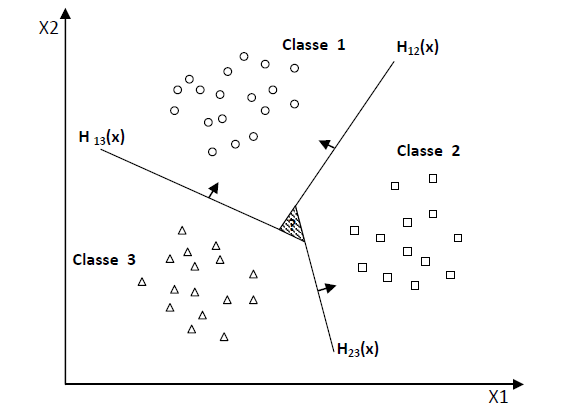
\includegraphics[width=10cm]{images/capt6}
	\caption{Approche une-contre-une}
\end{figure}
Bien que La méthode 1vs1 utilise, pour l’entrainement, un nombre plus important
d’hyperplans que la méthode 1vsR, elle est souvent plus rapide. Cela est du, d’une part,
au nombre limité d’exemples utilisés pour entrainer chaque hyperplan, et d’autre part, à la
simplicité des problèmes à résoudre. En effet, chaque deux classes prises à part sont moins
chevauchées que toutes les classes.


\chapter{Avantages et des inconvénients}
La méthode SVM présente des avantages et des inconvénients, comme toute méthode d'apprentissage automatique.

Les avantages de la méthode SVM sont les suivants :

Efficacité : la méthode SVM est très efficace pour résoudre les problèmes de classification et de régression, même pour les données de grande dimensionnalité.

Régularisation : la méthode SVM utilise une technique de régularisation qui permet d'éviter le surapprentissage, ce qui est particulièrement utile lorsque les données sont bruyantes ou déséquilibrées.

Adaptabilité : la méthode SVM est adaptable à différentes tâches de classification et de régression, grâce à l'utilisation de différents types de noyaux.

Interprétabilité : contrairement à certaines autres méthodes d'apprentissage automatique, la méthode SVM fournit une interprétation claire des résultats.

Robustesse : la méthode SVM est robuste aux données aberrantes, ce qui en fait une méthode utile pour les données bruyantes.

Cependant, la méthode SVM présente également quelques inconvénients, tels que :

Sensibilité au choix des paramètres : la méthode SVM est sensible au choix des paramètres, tels que le choix du noyau et les paramètres de régularisation.

Temps de calcul : la méthode SVM peut prendre beaucoup de temps de calcul pour les grands ensembles de données.

Difficulté à gérer les données manquantes : la méthode SVM a du mal à traiter les données manquantes ou incomplètes.

Pas approprié pour les problèmes de régression non linéaire : la méthode SVM est plus appropriée pour les problèmes de classification que pour les problèmes de régression non linéaire.


\chapter*{Conclusion}
\addcontentsline{toc}{chapter}{Conclusion}
En conclusion, la méthode SVM est une technique de classification puissante et efficace qui peut être utilisée dans de nombreux domaines, tels que la reconnaissance de formes, la vision par ordinateur, la bioinformatique et bien d'autres encore. Elle se distingue des autres méthodes de classification en utilisant des hyperplans pour séparer les données en classes distinctes.

La méthode SVM offre de nombreux avantages, tels que son efficacité pour résoudre les problèmes de classification, sa régularisation pour éviter le surapprentissage, sa capacité à gérer les données de grande dimensionnalité et sa robustesse aux données bruyantes. Cependant, elle a également quelques inconvénients, tels que sa sensibilité au choix des paramètres et son temps de calcul pour les grands ensembles de données.

Dans l'ensemble, la méthode SVM est une méthode très utile pour la classification, qui est largement utilisée dans de nombreux domaines. Elle a aidé les scientifiques, les ingénieurs et les professionnels de l'informatique à résoudre des problèmes complexes de classification avec succès. Cependant, il est important de comprendre les avantages et les inconvénients de la méthode SVM et de prendre en compte les spécificités de chaque problème de classification avant de choisir cette méthode pour résoudre un problème de classification donné.

	 %\begin{thebibliography}{9}
		%\bibitem{ref1} 
		
		
		
%	\end{thebibliography}
	
\end{document}